\section{Private-Public blockchain}
Publicly available software that ordinary people use every day is only a small fraction of all software. A lot of software and data is hidden behind corporate walls. Not every piece of information should be public and some of them are very sensitive. Companies often use software exclusively in their private networks to prevent unwanted data leaks or to protect themselves. Blockchain is no exception. It can be used worldwide where everyone can join the network and participate in the network as it can be used in a closed environment. Public and private blockchain share a lot of similarities. Both are decentralized P2P networks, where participants maintain a copy of a shared, synced append-only ledger of digitally signed transactions promising a guarantee if immutable data even when some participants are faulty or malicious. The main distinction between private and public is about who is allowed to participate in the network.
\begin{description}

\item[Public blockchain] is open to everyone willing to join. Even though everyone can join, participants in the network are completely anonymous. Everyone can download the whole blockchain and read the data. Currently the largest operational public blockchain network is the one behind Bitcoin. As of 2019, the current size of Bitcoin blockchain is more than 222 GB \cite{blockchain_size}. 

Public blockchains like Bitcoin consume an enormous amount of energy, time and money because of the mining and hence in return ensure trustlessness and remain tamper resistant. Bitcoin's current estimated annual electricity consumption is almost 50 TWh. About as much as Portugal uses in a year, worth around \$2,488,567,816  \cite{Bitcoin_Energy}. 


\begin{figure}[H]
    \begin{left}
        \begin{minipage}{\linewidth}
            \begin{left}
                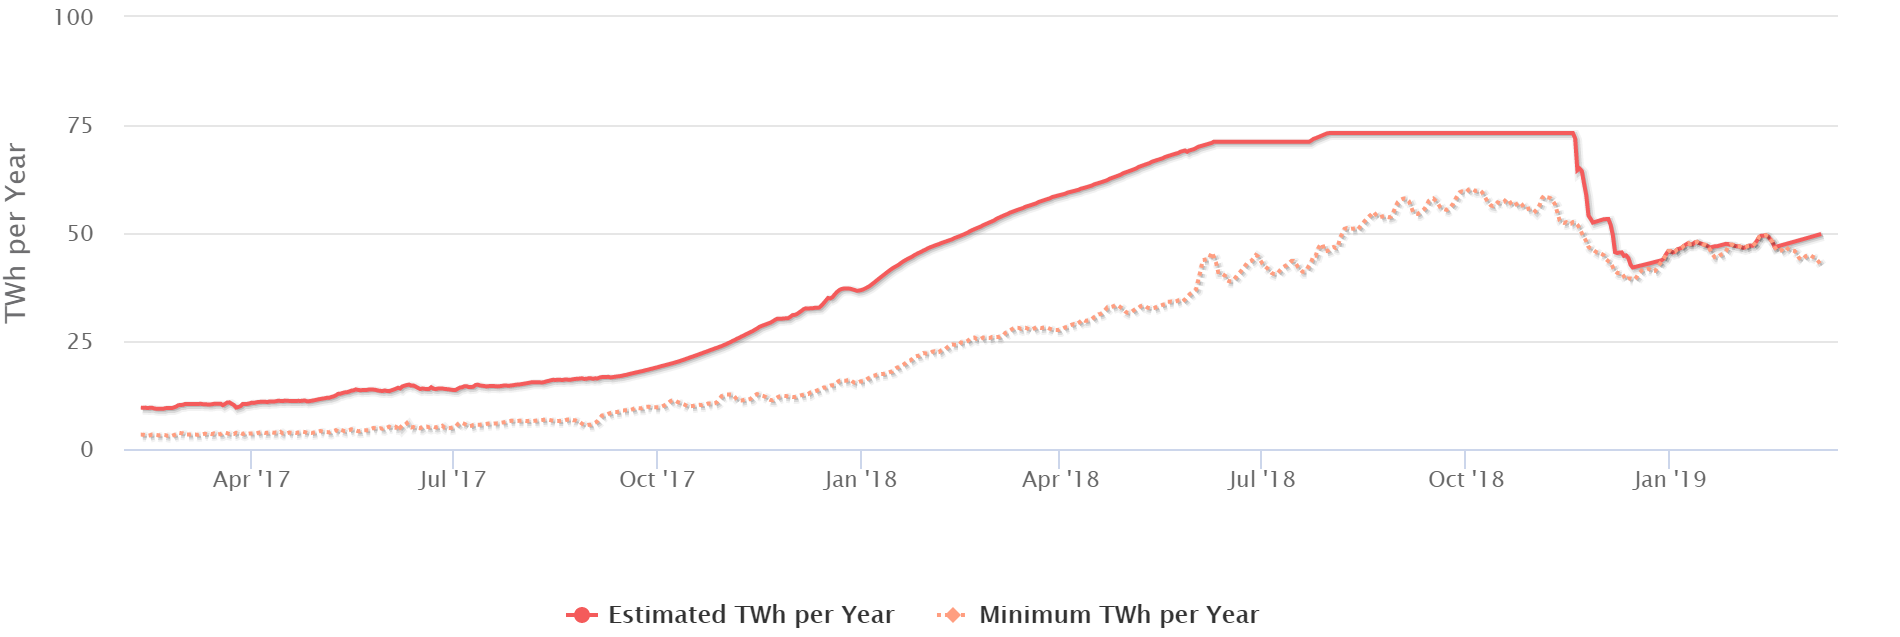
\includegraphics[width=\textwidth,keepaspectratio]{img/Bitcoin_Energy_Consumption_Index.png}
                \caption{Bitcoin Energy Consumption Index}
                \label{obr 1.3.1}
            \end{left}
        \end{minipage}
    \end{left}
\end{figure}



\item[Private blockchain] usually contains sensitive or internal information, therefore they're usually hosted in private network. Use of private blockchain is an answer to the enterprise use cases which requires performance characteristics that the permissionless blockchain technologies are unable to deliver.  

Following requirements for enterprise use of blockchain

\begin{itemize}
    \item Participants must be identified/identifiable
    \item Networks need to be permissioned
    \item High transaction throughput performance
    \item Low latency of transaction confirmation
    \item Privacy and confidentiality of transactions and data pertaining to business transactions
\end{itemize}


An invitation is required to join and new node must be validated by either the network starter or by a set of rules put in place by the network starter \cite{private_public_blockchain}. It's adding more security and transparency to help enterprises do business. Opposed to the public blockchain, private is much faster and cheaper because computers don't  have to spend an enormous amount of energy, time and money to reach a consensus. 
\end{description}
